\documentclass[11pt]{article}

\usepackage{url}
\usepackage[letterpaper,margin=1in]{geometry}
\usepackage{times}
\usepackage{graphicx}


\begin{document}

\title{My Great Project}
\author{John Sample \and Mary Joe}
\date{Final Project - CSCI 2950-u - Spring 2013}
\maketitle

\begin{abstract}
This is the abstract. This is the abstract. This is the abstract. 
This is the abstract. This is the abstract. This is the abstract. 
This is the abstract. This is the abstract. This is the abstract. 
This is the abstract. This is the abstract. This is the abstract. 
This is the abstract. This is the abstract. This is the abstract. 
\end{abstract}

\section{Introduction}
\label{sec:intro}
This is a simple example file on how to write a report using LaTeX.
Just use it as a base and replace the content. I put some examples of
commonly used features, but there are many more. Generally, you learn
these on demand. Examples include:

\begin{itemize}
\item Lists
\item Tables
\item Math text
\end{itemize}

After you write your LaTeX source, you have to compile it, run
BibTeX, and then compile twice again, to get all cross-references 
right. I also included a Makefile to make that whole process easier.
You just have to type \texttt{make} if you have your environment set.
It should work on Linux, MacOS, and cygwin. If you are running 
anything else, you should know how to set it up too.

Some sample text. Paragraphs are created by blank lines in the source.
Some sample text. Paragraphs are created by blank lines in the source.
Some sample text. Paragraphs are created by blank lines in the source.
Some sample text. Paragraphs are created by blank lines in the source.
Some sample text. Paragraphs are created by blank lines in the source.

Some sample text. Paragraphs are created by blank lines in the source.
Some sample text. Paragraphs are created by blank lines in the source.
Some sample text. Paragraphs are created by blank lines in the source.
Some sample text. Paragraphs are created by blank lines in the source.
Some sample text. Paragraphs are created by blank lines in the source.

\section{Another Section}

Another section. This one will have a figure. See
Figure~\ref{fig:us-versus-them}. Each figure has a label, which must be
defined \emph{after} the caption. Traditionally, people use
\texttt{fig:...} for figure labels, \texttt{sec:...} for section
labels, and \texttt{tab:...} for table labels. For example, this is a
reference to Section~\ref{sec:intro}. 

\begin{figure}
\centering
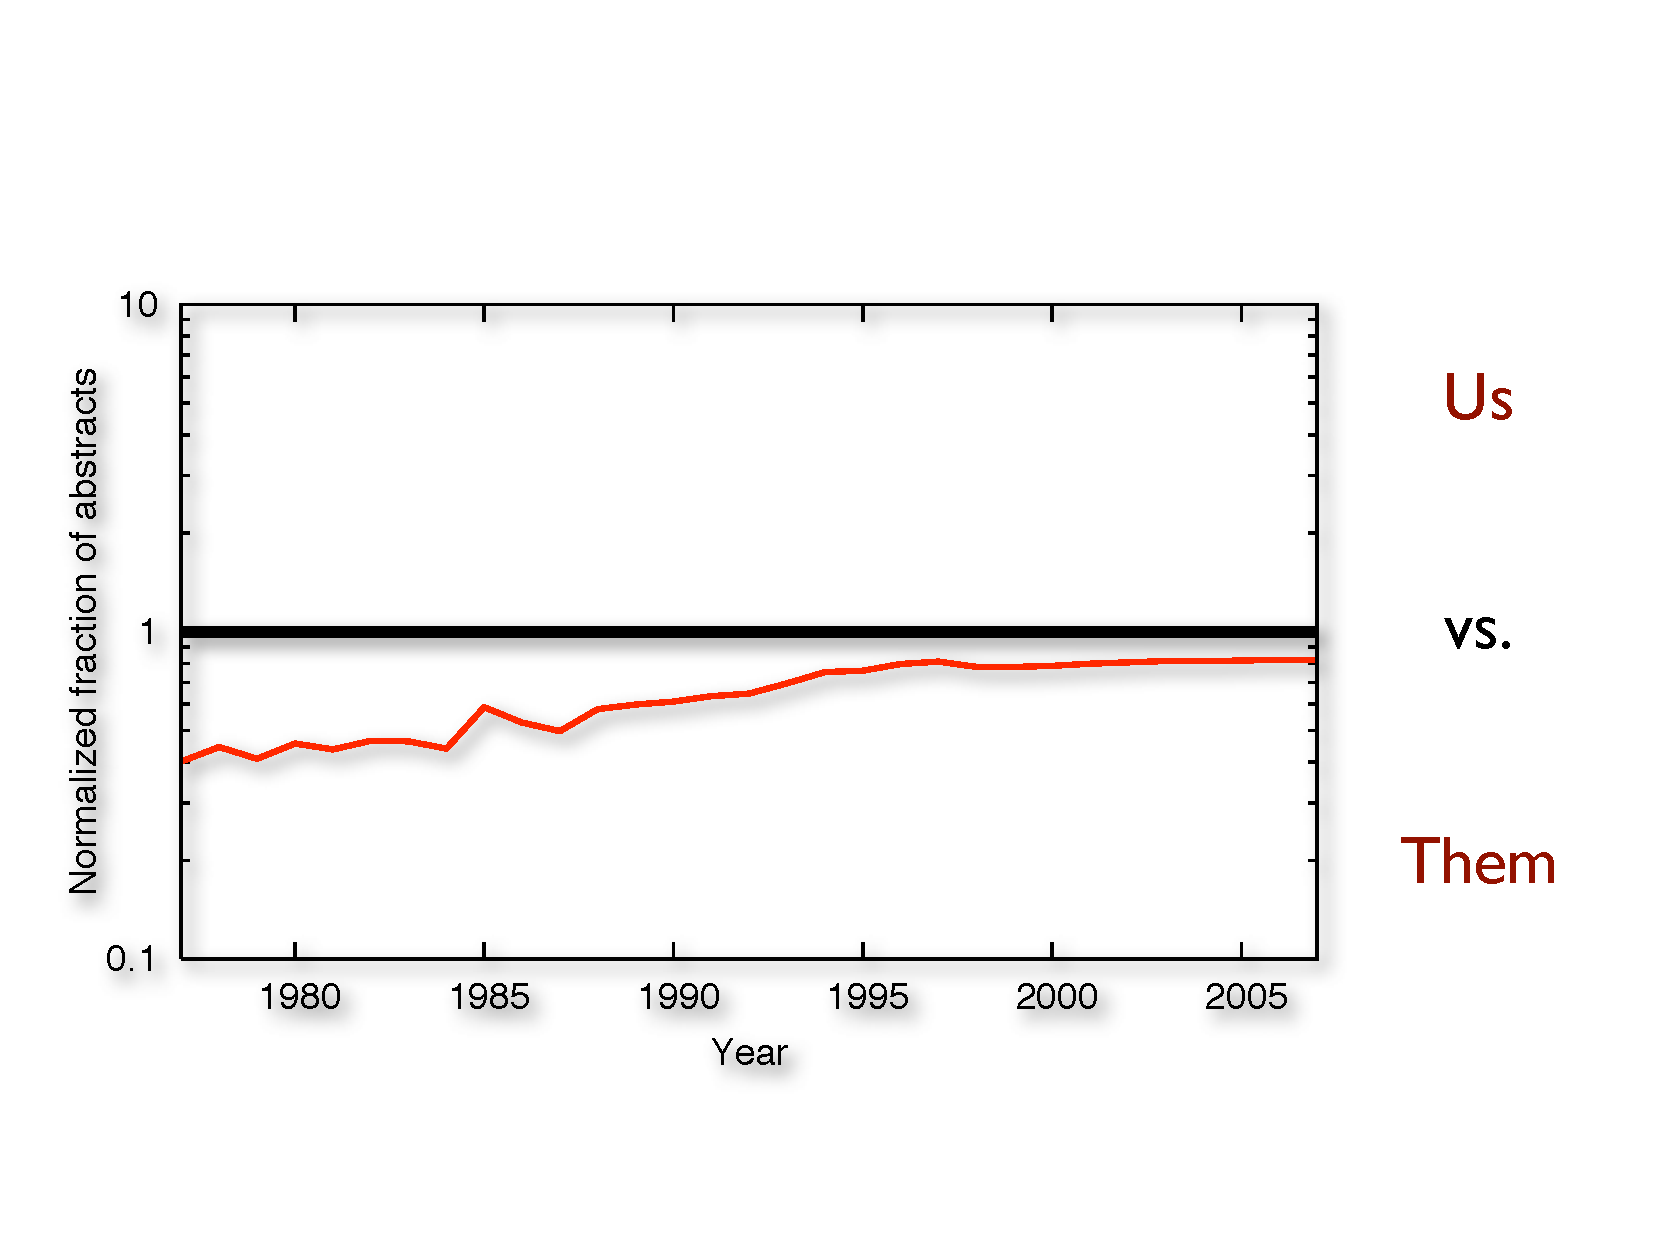
\includegraphics[width=0.7\textwidth]{usthem}
\caption{Relative number of abstracts from the ACM Digital Library
containing the word `us' versus the word 'them'. According
to~\cite{godfrey08}, `they are winning, but we are gaining on Them'. }
\label{fig:us-versus-them}
\end{figure}

\section{Related Work}

A nice feature for collaboration is that you can break your document
into many files with \texttt{\\input}, and have each person work on a
different file. This works great if you have some sort of version
control such as SVN or GIT.

Finally, you may want to cite some previous work. For
example,~\cite{lamport78time} is a highly-cited paper.
The ACM digital library is a good source of BibTeX entries.

% This is a comment: if you are curious, the ~ before \cite is a
% non-breaking space: it produces a space before the citation and
% doesn't let it go to the beginning of the next line if it would
% cause a line break.




\section{Conclusions}

It should be easy to write your report in LaTeX, and it's a great tool
to learn. It almost certainly came with your Linux installation, and
can be very easily installed in Cygwin and on the Mac (through the
excellent MacTeX distribution).


\bibliographystyle{plain}
\bibliography{report}

\end{document}
